\documentclass[11pt]{article}
% ---------------------------------------------------------------
% R3.07 SQL dans un langage de programmation -- preambule commun des sujets de TP
% Article clair, fond blanc, accents de couleur coherents avec les slides
% Charte derivee de R5.A.08 Qualite de developpement (meme palette IUT)
% Utilisation :
%   \documentclass[11pt]{article}
%   % ---------------------------------------------------------------
% R3.07 SQL dans un langage de programmation -- preambule commun des sujets de TP
% Article clair, fond blanc, accents de couleur coherents avec les slides
% Charte derivee de R5.A.08 Qualite de developpement (meme palette IUT)
% Utilisation :
%   \documentclass[11pt]{article}
%   % ---------------------------------------------------------------
% R3.07 SQL dans un langage de programmation -- preambule commun des sujets de TP
% Article clair, fond blanc, accents de couleur coherents avec les slides
% Charte derivee de R5.A.08 Qualite de developpement (meme palette IUT)
% Utilisation :
%   \documentclass[11pt]{article}
%   \input{../../latex/common/r307-tp-preamble.tex}
%   \begin{document}
%   \rtpheader{1}{Titre du TP}
% ---------------------------------------------------------------
\usepackage[T1]{fontenc}
\usepackage[utf8]{inputenc}
\usepackage[french]{babel}
\usepackage[scale=0.92]{tgheros}
\usepackage{tgpagella}
\usepackage[a4paper, margin=2.2cm, headheight=14pt]{geometry}
\usepackage{graphicx}
\usepackage{xcolor}
\usepackage{listings}
\usepackage[skins,listings,breakable]{tcolorbox}
\usepackage{enumitem}
\usepackage{booktabs}
\usepackage{array}
\usepackage{multirow}
\usepackage{tikz}
\usetikzlibrary{shapes, shapes.geometric, arrows, arrows.meta, positioning, calc}
\usepackage[colorlinks=true, linkcolor=qaaccentdark, urlcolor=qaaccentdark]{hyperref}
\usepackage{fancyhdr}
\usepackage{lastpage}
\usepackage{titlesec}
\usepackage{etoolbox}

% ---------------------------------------------------------------
% PALETTE -- version imprimable des couleurs des diapositives
% ---------------------------------------------------------------
\definecolor{qaaccentdark}{HTML}{7A1680}   % violet du logo IUT, fonce pour rester lisible sur blanc
\definecolor{qaaccent2dark}{HTML}{9B4B94}  % violet clair du logo IUT (accent secondaire)
\definecolor{qapanellight}{HTML}{F4F6F8}   % fond de bloc tres clair
\definecolor{qalinelight}{HTML}{D8DEE4}    % filets
\definecolor{qatextdark}{HTML}{1A1D23}     % texte principal
\definecolor{qamuteddark}{HTML}{5B6472}    % texte secondaire
\definecolor{qacodekwl}{HTML}{7A1680}      % code : mots-cles
\definecolor{qacodestrl}{HTML}{2E7D32}     % code : chaines
\definecolor{qacodecoml}{HTML}{6B7280}     % code : commentaires
\definecolor{qacodeannl}{HTML}{B26A00}     % code : annotations / javadoc

\color{qatextdark}

\setlength{\parskip}{4pt}
\setlength{\parindent}{0pt}

% ---------------------------------------------------------------
% TITRES DE SECTION -- texte blanc sur bande de couleur pleine largeur
% (gere aussi les variantes etoilees \section*)
% ---------------------------------------------------------------
\newcommand{\qasectionband}[2]{%
  \noindent\colorbox{#1}{%
    \parbox[c]{\dimexpr\linewidth-2\fboxsep\relax}{%
      \color{white}#2%
    }%
  }%
}
\newcommand{\secformat}[1]{\qasectionband{qaaccentdark}{\bfseries\Large\thesection\quad #1}}
\newcommand{\secformatnn}[1]{\qasectionband{qaaccentdark}{\bfseries\Large #1}}
\newcommand{\subsecformat}[1]{\qasectionband{qaaccent2dark}{\bfseries\large\thesubsection\quad #1}}
\newcommand{\subsecformatnn}[1]{\qasectionband{qaaccent2dark}{\bfseries\large #1}}

\titleformat{\section}{\normalfont}{}{0pt}{\secformat}
\titleformat{name=\section,numberless}{\normalfont}{}{0pt}{\secformatnn}
\titleformat{\subsection}{\normalfont}{}{0pt}{\subsecformat}
\titleformat{name=\subsection,numberless}{\normalfont}{}{0pt}{\subsecformatnn}
\titleformat{\subsubsection}{\normalfont\bfseries\color{qaaccentdark}}{\thesubsubsection}{0.6em}{}
\titlespacing*{\section}{0pt}{14pt}{8pt}
\titlespacing*{\subsection}{0pt}{10pt}{6pt}
\titlespacing*{\subsubsection}{0pt}{8pt}{4pt}

% ---------------------------------------------------------------
% LISTINGS -- theme clair (lstlisting reste utilisable tel quel)
% \lstcode : police + couleur de base, a reutiliser dans les surcharges
% ---------------------------------------------------------------
\newcommand{\lstcode}{\ttfamily\color{qatextdark}}

\lstdefinelanguage{TypeScript}{
  keywords={typeof, new, true, false, catch, function, return, null, switch, var,
    if, in, while, do, else, case, break, const, let, interface, class, extends,
    implements, enum, export, import, this, super, constructor, public, private,
    protected, static, async, await, throw, throws, try, finally, void},
  ndkeywords={boolean, any, number, string, int, long, double},
  sensitive=true,
  comment=[l]{//},
  morecomment=[s]{/*}{*/},
  morestring=[b]',
  morestring=[b]"
}

\lstdefinestyle{r307code}{
  basicstyle=\lstcode\footnotesize,
  keywordstyle=\color{qacodekwl}\bfseries,
  ndkeywordstyle=\color{qaaccent2dark}\bfseries,
  stringstyle=\color{qacodestrl},
  commentstyle=\color{qacodecoml}\itshape,
  morecomment=[s][\color{qacodeannl}]{/**}{*/},
  backgroundcolor=\color{qapanellight},
  rulecolor=\color{qalinelight},
  frame=single,
  framesep=4pt,
  xleftmargin=6pt,
  xrightmargin=6pt,
  numbers=left,
  numberstyle=\tiny\color{qamuteddark},
  numbersep=8pt,
  keepspaces=true,
  columns=fullflexible,
  showstringspaces=false,
  showspaces=false,
  showtabs=false,
  breaklines=true,
  breakatwhitespace=false,
  captionpos=b,
  tabsize=2,
  escapeinside={(*@}{@*)},
}
\lstset{style=r307code}

% ---------------------------------------------------------------
% BOITES : exercice, code, information
% ---------------------------------------------------------------
\tcbset{
  exobox/.style={colback=qapanellight, colframe=qaaccentdark, boxrule=0.6pt,
    arc=2pt, left=8pt, right=8pt, top=6pt, bottom=6pt,
    coltitle=white, colbacktitle=qaaccentdark, fonttitle=\bfseries,
    boxsep=2pt, breakable},
  infobox/.style={colback=white, colframe=qaaccent2dark, boxrule=0.6pt,
    leftrule=3pt, arc=0pt, left=8pt, right=8pt, top=5pt, bottom=5pt,
    coltitle=qaaccent2dark, colbacktitle=white, fonttitle=\bfseries,
    breakable},
  codebox/.style={colback=qatextdark, colframe=qalinelight, boxrule=0.4pt,
    arc=2pt, left=8pt, right=8pt, top=5pt, bottom=5pt, listing only,
    listing options={basicstyle=\ttfamily\small\color{white},
      breaklines=true, showstringspaces=false, columns=fullflexible,
      keepspaces=true, frame=none, numbers=none, backgroundcolor={}}, breakable}
}
\newtcolorbox[auto counter]{exobox}[2][]{exobox,
  title={Exercice~\thetcbcounter\ifstrempty{#2}{}{ --- #2}}, #1}
\newtcolorbox{infobox}[1][\`A retenir]{infobox, title={#1}}
\newtcblisting{codebox}{codebox}

% ---------------------------------------------------------------
% EN-TETE DE PAGE (fil d'Ariane + pagination)
% ---------------------------------------------------------------
\newcommand{\qaheadtitlevalue}{}
\newcommand{\qaheadtitle}[1]{\renewcommand{\qaheadtitlevalue}{#1}}

\pagestyle{fancy}
\fancyhf{}
\renewcommand{\headrulewidth}{0.4pt}
\fancyhead[L]{\small\color{qamuteddark}R3.07 --- \qaheadtitlevalue}
\fancyhead[R]{\small\color{qamuteddark}\thepage\,/\,\pageref{LastPage}}
\fancyfoot[C]{\footnotesize\color{qamuteddark}IUT de Vannes --- Universit\'e Bretagne Sud}
\fancypagestyle{plain}{\fancyhf{}\renewcommand{\headrulewidth}{0pt}%
  \fancyfoot[C]{\footnotesize\color{qamuteddark}IUT de Vannes --- Universit\'e Bretagne Sud}}

% ---------------------------------------------------------------
% BANDEAU DE TITRE (pas une page dediee, pour rester compact)
% \rtpheader{numero ou intitule court}{titre du TP}
% ---------------------------------------------------------------
\newcommand{\ryear}{2026/2027}
\newcommand{\rtpheader}[2]{%
  \thispagestyle{plain}%
  \begin{minipage}[t]{0.68\textwidth}
    {\small\color{qamuteddark}
      Universit\'e Bretagne Sud\\
      IUT de Vannes\\
      D\'epartement Informatique --- \ryear}
  \end{minipage}%
  \hfill
  \begin{minipage}[t]{0.28\textwidth}
    \raggedleft
    \includegraphics[width=2.6cm]{iut_logo.jpg}
  \end{minipage}

  \vspace{6mm}
  \begin{center}
    {\large\bfseries\color{qatextdark} BUT 2 --- R3.07. SQL dans un langage de programmation}\\[2mm]
    {\normalsize\color{qamuteddark} TD/TP #1}\\[1mm]
    {\Large\bfseries\color{qaaccentdark} #2}
  \end{center}
  \vspace{4mm}
  \qaheadtitle{#2}
}

%   \begin{document}
%   \rtpheader{1}{Titre du TP}
% ---------------------------------------------------------------
\usepackage[T1]{fontenc}
\usepackage[utf8]{inputenc}
\usepackage[french]{babel}
\usepackage[scale=0.92]{tgheros}
\usepackage{tgpagella}
\usepackage[a4paper, margin=2.2cm, headheight=14pt]{geometry}
\usepackage{graphicx}
\usepackage{xcolor}
\usepackage{listings}
\usepackage[skins,listings,breakable]{tcolorbox}
\usepackage{enumitem}
\usepackage{booktabs}
\usepackage{array}
\usepackage{multirow}
\usepackage{tikz}
\usetikzlibrary{shapes, shapes.geometric, arrows, arrows.meta, positioning, calc}
\usepackage[colorlinks=true, linkcolor=qaaccentdark, urlcolor=qaaccentdark]{hyperref}
\usepackage{fancyhdr}
\usepackage{lastpage}
\usepackage{titlesec}
\usepackage{etoolbox}

% ---------------------------------------------------------------
% PALETTE -- version imprimable des couleurs des diapositives
% ---------------------------------------------------------------
\definecolor{qaaccentdark}{HTML}{7A1680}   % violet du logo IUT, fonce pour rester lisible sur blanc
\definecolor{qaaccent2dark}{HTML}{9B4B94}  % violet clair du logo IUT (accent secondaire)
\definecolor{qapanellight}{HTML}{F4F6F8}   % fond de bloc tres clair
\definecolor{qalinelight}{HTML}{D8DEE4}    % filets
\definecolor{qatextdark}{HTML}{1A1D23}     % texte principal
\definecolor{qamuteddark}{HTML}{5B6472}    % texte secondaire
\definecolor{qacodekwl}{HTML}{7A1680}      % code : mots-cles
\definecolor{qacodestrl}{HTML}{2E7D32}     % code : chaines
\definecolor{qacodecoml}{HTML}{6B7280}     % code : commentaires
\definecolor{qacodeannl}{HTML}{B26A00}     % code : annotations / javadoc

\color{qatextdark}

\setlength{\parskip}{4pt}
\setlength{\parindent}{0pt}

% ---------------------------------------------------------------
% TITRES DE SECTION -- texte blanc sur bande de couleur pleine largeur
% (gere aussi les variantes etoilees \section*)
% ---------------------------------------------------------------
\newcommand{\qasectionband}[2]{%
  \noindent\colorbox{#1}{%
    \parbox[c]{\dimexpr\linewidth-2\fboxsep\relax}{%
      \color{white}#2%
    }%
  }%
}
\newcommand{\secformat}[1]{\qasectionband{qaaccentdark}{\bfseries\Large\thesection\quad #1}}
\newcommand{\secformatnn}[1]{\qasectionband{qaaccentdark}{\bfseries\Large #1}}
\newcommand{\subsecformat}[1]{\qasectionband{qaaccent2dark}{\bfseries\large\thesubsection\quad #1}}
\newcommand{\subsecformatnn}[1]{\qasectionband{qaaccent2dark}{\bfseries\large #1}}

\titleformat{\section}{\normalfont}{}{0pt}{\secformat}
\titleformat{name=\section,numberless}{\normalfont}{}{0pt}{\secformatnn}
\titleformat{\subsection}{\normalfont}{}{0pt}{\subsecformat}
\titleformat{name=\subsection,numberless}{\normalfont}{}{0pt}{\subsecformatnn}
\titleformat{\subsubsection}{\normalfont\bfseries\color{qaaccentdark}}{\thesubsubsection}{0.6em}{}
\titlespacing*{\section}{0pt}{14pt}{8pt}
\titlespacing*{\subsection}{0pt}{10pt}{6pt}
\titlespacing*{\subsubsection}{0pt}{8pt}{4pt}

% ---------------------------------------------------------------
% LISTINGS -- theme clair (lstlisting reste utilisable tel quel)
% \lstcode : police + couleur de base, a reutiliser dans les surcharges
% ---------------------------------------------------------------
\newcommand{\lstcode}{\ttfamily\color{qatextdark}}

\lstdefinelanguage{TypeScript}{
  keywords={typeof, new, true, false, catch, function, return, null, switch, var,
    if, in, while, do, else, case, break, const, let, interface, class, extends,
    implements, enum, export, import, this, super, constructor, public, private,
    protected, static, async, await, throw, throws, try, finally, void},
  ndkeywords={boolean, any, number, string, int, long, double},
  sensitive=true,
  comment=[l]{//},
  morecomment=[s]{/*}{*/},
  morestring=[b]',
  morestring=[b]"
}

\lstdefinestyle{r307code}{
  basicstyle=\lstcode\footnotesize,
  keywordstyle=\color{qacodekwl}\bfseries,
  ndkeywordstyle=\color{qaaccent2dark}\bfseries,
  stringstyle=\color{qacodestrl},
  commentstyle=\color{qacodecoml}\itshape,
  morecomment=[s][\color{qacodeannl}]{/**}{*/},
  backgroundcolor=\color{qapanellight},
  rulecolor=\color{qalinelight},
  frame=single,
  framesep=4pt,
  xleftmargin=6pt,
  xrightmargin=6pt,
  numbers=left,
  numberstyle=\tiny\color{qamuteddark},
  numbersep=8pt,
  keepspaces=true,
  columns=fullflexible,
  showstringspaces=false,
  showspaces=false,
  showtabs=false,
  breaklines=true,
  breakatwhitespace=false,
  captionpos=b,
  tabsize=2,
  escapeinside={(*@}{@*)},
}
\lstset{style=r307code}

% ---------------------------------------------------------------
% BOITES : exercice, code, information
% ---------------------------------------------------------------
\tcbset{
  exobox/.style={colback=qapanellight, colframe=qaaccentdark, boxrule=0.6pt,
    arc=2pt, left=8pt, right=8pt, top=6pt, bottom=6pt,
    coltitle=white, colbacktitle=qaaccentdark, fonttitle=\bfseries,
    boxsep=2pt, breakable},
  infobox/.style={colback=white, colframe=qaaccent2dark, boxrule=0.6pt,
    leftrule=3pt, arc=0pt, left=8pt, right=8pt, top=5pt, bottom=5pt,
    coltitle=qaaccent2dark, colbacktitle=white, fonttitle=\bfseries,
    breakable},
  codebox/.style={colback=qatextdark, colframe=qalinelight, boxrule=0.4pt,
    arc=2pt, left=8pt, right=8pt, top=5pt, bottom=5pt, listing only,
    listing options={basicstyle=\ttfamily\small\color{white},
      breaklines=true, showstringspaces=false, columns=fullflexible,
      keepspaces=true, frame=none, numbers=none, backgroundcolor={}}, breakable}
}
\newtcolorbox[auto counter]{exobox}[2][]{exobox,
  title={Exercice~\thetcbcounter\ifstrempty{#2}{}{ --- #2}}, #1}
\newtcolorbox{infobox}[1][\`A retenir]{infobox, title={#1}}
\newtcblisting{codebox}{codebox}

% ---------------------------------------------------------------
% EN-TETE DE PAGE (fil d'Ariane + pagination)
% ---------------------------------------------------------------
\newcommand{\qaheadtitlevalue}{}
\newcommand{\qaheadtitle}[1]{\renewcommand{\qaheadtitlevalue}{#1}}

\pagestyle{fancy}
\fancyhf{}
\renewcommand{\headrulewidth}{0.4pt}
\fancyhead[L]{\small\color{qamuteddark}R3.07 --- \qaheadtitlevalue}
\fancyhead[R]{\small\color{qamuteddark}\thepage\,/\,\pageref{LastPage}}
\fancyfoot[C]{\footnotesize\color{qamuteddark}IUT de Vannes --- Universit\'e Bretagne Sud}
\fancypagestyle{plain}{\fancyhf{}\renewcommand{\headrulewidth}{0pt}%
  \fancyfoot[C]{\footnotesize\color{qamuteddark}IUT de Vannes --- Universit\'e Bretagne Sud}}

% ---------------------------------------------------------------
% BANDEAU DE TITRE (pas une page dediee, pour rester compact)
% \rtpheader{numero ou intitule court}{titre du TP}
% ---------------------------------------------------------------
\newcommand{\ryear}{2026/2027}
\newcommand{\rtpheader}[2]{%
  \thispagestyle{plain}%
  \begin{minipage}[t]{0.68\textwidth}
    {\small\color{qamuteddark}
      Universit\'e Bretagne Sud\\
      IUT de Vannes\\
      D\'epartement Informatique --- \ryear}
  \end{minipage}%
  \hfill
  \begin{minipage}[t]{0.28\textwidth}
    \raggedleft
    \includegraphics[width=2.6cm]{iut_logo.jpg}
  \end{minipage}

  \vspace{6mm}
  \begin{center}
    {\large\bfseries\color{qatextdark} BUT 2 --- R3.07. SQL dans un langage de programmation}\\[2mm]
    {\normalsize\color{qamuteddark} TD/TP #1}\\[1mm]
    {\Large\bfseries\color{qaaccentdark} #2}
  \end{center}
  \vspace{4mm}
  \qaheadtitle{#2}
}

%   \begin{document}
%   \rtpheader{1}{Titre du TP}
% ---------------------------------------------------------------
\usepackage[T1]{fontenc}
\usepackage[utf8]{inputenc}
\usepackage[french]{babel}
\usepackage[scale=0.92]{tgheros}
\usepackage{tgpagella}
\usepackage[a4paper, margin=2.2cm, headheight=14pt]{geometry}
\usepackage{graphicx}
\usepackage{xcolor}
\usepackage{listings}
\usepackage[skins,listings,breakable]{tcolorbox}
\usepackage{enumitem}
\usepackage{booktabs}
\usepackage{array}
\usepackage{multirow}
\usepackage{tikz}
\usetikzlibrary{shapes, shapes.geometric, arrows, arrows.meta, positioning, calc}
\usepackage[colorlinks=true, linkcolor=qaaccentdark, urlcolor=qaaccentdark]{hyperref}
\usepackage{fancyhdr}
\usepackage{lastpage}
\usepackage{titlesec}
\usepackage{etoolbox}

% ---------------------------------------------------------------
% PALETTE -- version imprimable des couleurs des diapositives
% ---------------------------------------------------------------
\definecolor{qaaccentdark}{HTML}{7A1680}   % violet du logo IUT, fonce pour rester lisible sur blanc
\definecolor{qaaccent2dark}{HTML}{9B4B94}  % violet clair du logo IUT (accent secondaire)
\definecolor{qapanellight}{HTML}{F4F6F8}   % fond de bloc tres clair
\definecolor{qalinelight}{HTML}{D8DEE4}    % filets
\definecolor{qatextdark}{HTML}{1A1D23}     % texte principal
\definecolor{qamuteddark}{HTML}{5B6472}    % texte secondaire
\definecolor{qacodekwl}{HTML}{7A1680}      % code : mots-cles
\definecolor{qacodestrl}{HTML}{2E7D32}     % code : chaines
\definecolor{qacodecoml}{HTML}{6B7280}     % code : commentaires
\definecolor{qacodeannl}{HTML}{B26A00}     % code : annotations / javadoc

\color{qatextdark}

\setlength{\parskip}{4pt}
\setlength{\parindent}{0pt}

% ---------------------------------------------------------------
% TITRES DE SECTION -- texte blanc sur bande de couleur pleine largeur
% (gere aussi les variantes etoilees \section*)
% ---------------------------------------------------------------
\newcommand{\qasectionband}[2]{%
  \noindent\colorbox{#1}{%
    \parbox[c]{\dimexpr\linewidth-2\fboxsep\relax}{%
      \color{white}#2%
    }%
  }%
}
\newcommand{\secformat}[1]{\qasectionband{qaaccentdark}{\bfseries\Large\thesection\quad #1}}
\newcommand{\secformatnn}[1]{\qasectionband{qaaccentdark}{\bfseries\Large #1}}
\newcommand{\subsecformat}[1]{\qasectionband{qaaccent2dark}{\bfseries\large\thesubsection\quad #1}}
\newcommand{\subsecformatnn}[1]{\qasectionband{qaaccent2dark}{\bfseries\large #1}}

\titleformat{\section}{\normalfont}{}{0pt}{\secformat}
\titleformat{name=\section,numberless}{\normalfont}{}{0pt}{\secformatnn}
\titleformat{\subsection}{\normalfont}{}{0pt}{\subsecformat}
\titleformat{name=\subsection,numberless}{\normalfont}{}{0pt}{\subsecformatnn}
\titleformat{\subsubsection}{\normalfont\bfseries\color{qaaccentdark}}{\thesubsubsection}{0.6em}{}
\titlespacing*{\section}{0pt}{14pt}{8pt}
\titlespacing*{\subsection}{0pt}{10pt}{6pt}
\titlespacing*{\subsubsection}{0pt}{8pt}{4pt}

% ---------------------------------------------------------------
% LISTINGS -- theme clair (lstlisting reste utilisable tel quel)
% \lstcode : police + couleur de base, a reutiliser dans les surcharges
% ---------------------------------------------------------------
\newcommand{\lstcode}{\ttfamily\color{qatextdark}}

\lstdefinelanguage{TypeScript}{
  keywords={typeof, new, true, false, catch, function, return, null, switch, var,
    if, in, while, do, else, case, break, const, let, interface, class, extends,
    implements, enum, export, import, this, super, constructor, public, private,
    protected, static, async, await, throw, throws, try, finally, void},
  ndkeywords={boolean, any, number, string, int, long, double},
  sensitive=true,
  comment=[l]{//},
  morecomment=[s]{/*}{*/},
  morestring=[b]',
  morestring=[b]"
}

\lstdefinestyle{r307code}{
  basicstyle=\lstcode\footnotesize,
  keywordstyle=\color{qacodekwl}\bfseries,
  ndkeywordstyle=\color{qaaccent2dark}\bfseries,
  stringstyle=\color{qacodestrl},
  commentstyle=\color{qacodecoml}\itshape,
  morecomment=[s][\color{qacodeannl}]{/**}{*/},
  backgroundcolor=\color{qapanellight},
  rulecolor=\color{qalinelight},
  frame=single,
  framesep=4pt,
  xleftmargin=6pt,
  xrightmargin=6pt,
  numbers=left,
  numberstyle=\tiny\color{qamuteddark},
  numbersep=8pt,
  keepspaces=true,
  columns=fullflexible,
  showstringspaces=false,
  showspaces=false,
  showtabs=false,
  breaklines=true,
  breakatwhitespace=false,
  captionpos=b,
  tabsize=2,
  escapeinside={(*@}{@*)},
}
\lstset{style=r307code}

% ---------------------------------------------------------------
% BOITES : exercice, code, information
% ---------------------------------------------------------------
\tcbset{
  exobox/.style={colback=qapanellight, colframe=qaaccentdark, boxrule=0.6pt,
    arc=2pt, left=8pt, right=8pt, top=6pt, bottom=6pt,
    coltitle=white, colbacktitle=qaaccentdark, fonttitle=\bfseries,
    boxsep=2pt, breakable},
  infobox/.style={colback=white, colframe=qaaccent2dark, boxrule=0.6pt,
    leftrule=3pt, arc=0pt, left=8pt, right=8pt, top=5pt, bottom=5pt,
    coltitle=qaaccent2dark, colbacktitle=white, fonttitle=\bfseries,
    breakable},
  codebox/.style={colback=qatextdark, colframe=qalinelight, boxrule=0.4pt,
    arc=2pt, left=8pt, right=8pt, top=5pt, bottom=5pt, listing only,
    listing options={basicstyle=\ttfamily\small\color{white},
      breaklines=true, showstringspaces=false, columns=fullflexible,
      keepspaces=true, frame=none, numbers=none, backgroundcolor={}}, breakable}
}
\newtcolorbox[auto counter]{exobox}[2][]{exobox,
  title={Exercice~\thetcbcounter\ifstrempty{#2}{}{ --- #2}}, #1}
\newtcolorbox{infobox}[1][\`A retenir]{infobox, title={#1}}
\newtcblisting{codebox}{codebox}

% ---------------------------------------------------------------
% EN-TETE DE PAGE (fil d'Ariane + pagination)
% ---------------------------------------------------------------
\newcommand{\qaheadtitlevalue}{}
\newcommand{\qaheadtitle}[1]{\renewcommand{\qaheadtitlevalue}{#1}}

\pagestyle{fancy}
\fancyhf{}
\renewcommand{\headrulewidth}{0.4pt}
\fancyhead[L]{\small\color{qamuteddark}R3.07 --- \qaheadtitlevalue}
\fancyhead[R]{\small\color{qamuteddark}\thepage\,/\,\pageref{LastPage}}
\fancyfoot[C]{\footnotesize\color{qamuteddark}IUT de Vannes --- Universit\'e Bretagne Sud}
\fancypagestyle{plain}{\fancyhf{}\renewcommand{\headrulewidth}{0pt}%
  \fancyfoot[C]{\footnotesize\color{qamuteddark}IUT de Vannes --- Universit\'e Bretagne Sud}}

% ---------------------------------------------------------------
% BANDEAU DE TITRE (pas une page dediee, pour rester compact)
% \rtpheader{numero ou intitule court}{titre du TP}
% ---------------------------------------------------------------
\newcommand{\ryear}{2026/2027}
\newcommand{\rtpheader}[2]{%
  \thispagestyle{plain}%
  \begin{minipage}[t]{0.68\textwidth}
    {\small\color{qamuteddark}
      Universit\'e Bretagne Sud\\
      IUT de Vannes\\
      D\'epartement Informatique --- \ryear}
  \end{minipage}%
  \hfill
  \begin{minipage}[t]{0.28\textwidth}
    \raggedleft
    \includegraphics[width=2.6cm]{iut_logo.jpg}
  \end{minipage}

  \vspace{6mm}
  \begin{center}
    {\large\bfseries\color{qatextdark} BUT 2 --- R3.07. SQL dans un langage de programmation}\\[2mm]
    {\normalsize\color{qamuteddark} TD/TP #1}\\[1mm]
    {\Large\bfseries\color{qaaccentdark} #2}
  \end{center}
  \vspace{4mm}
  \qaheadtitle{#2}
}

\graphicspath{{../../latex/common/assets/}{./}}


\begin{document}

\rtpheader{1}{Acc\`es \`a une base de donn\'ees avec JDBC}

	
\section{Introduction}
Dans ce TD/TP, vous allez développer une application Java qui interagit avec une base de données relationnelle en utilisant JDBC. Vous devrez également dockeriser votre application et la base de données.

\section{Prérequis}
\begin{itemize}
    \item Connaissances de base en Java.
    \item Docker installé sur votre machine et une bonne connexion Internet.
    \item L'IDE IntelliJ IDEA de Jetbrains.
\end{itemize}

\section{Diagramme de la base de données}
\begin{center}
    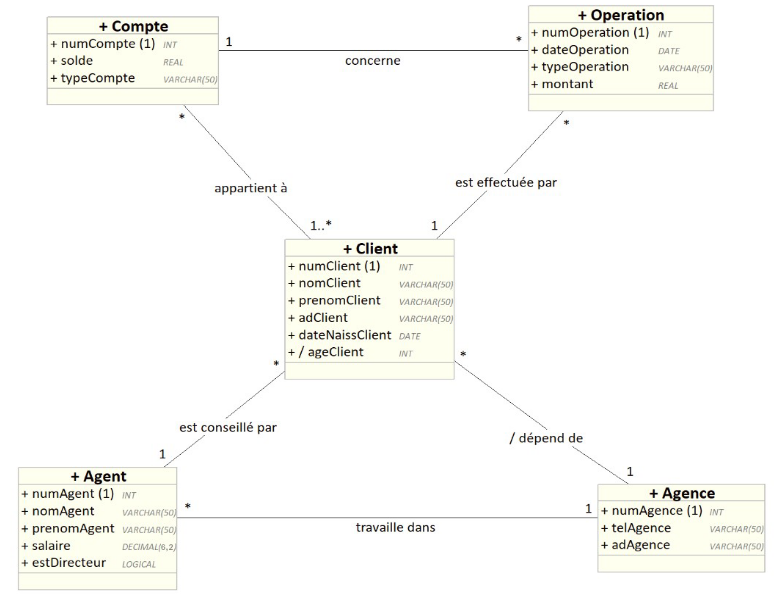
\includegraphics[width=1\textwidth]{img/db_schema.png}
\end{center}

\section{Description de la base de données}
Le schéma de la base de données est le suivant :
\begin{itemize}
    \item \textbf{Compte} : numCompte (INT), solde (REAL), typeCompte (VARCHAR).
    \item \textbf{Client} : numClient (INT), nomClient (VARCHAR), prenomClient (VARCHAR), adClient (VARCHAR), dateNaissClient (DATE), ageClient (INT).
    \item \textbf{Opération} : numOperation (INT), dateOperation (DATE), typeOperation (VARCHAR), montant (REAL).
    \item \textbf{Agent} : numAgent (INT), nomAgent (VARCHAR), prenomAgent (VARCHAR), salaire (DECIMAL), estDirecteur (LOGICAL).
    \item \textbf{Agence} : numAgence (INT), telAgence (VARCHAR), adAgence (VARCHAR).
\end{itemize}

\section{Mise en place de la base de données avec Docker}
Vous allez utiliser Docker pour créer une instance PostgreSQL contenant cette base de données.

\subsection{Étape 1 : Créer un docker-compose.yml pour la base de données}
Créez un fichier \texttt{docker-compose.yml} pour lancer un conteneur PostgreSQL avec la base de données initialisée.

\begin{lstlisting}
version: '3.8'
services:
  db:
    image: postgres:18
    environment:
      POSTGRES_USER: user
      POSTGRES_PASSWORD: password
      POSTGRES_DB: banque_db
    ports:
      - "5432:5432"
    volumes:
      - ./init.sql:/docker-entrypoint-initdb.d/init.sql
\end{lstlisting}

\subsection{Étape 2 : Script SQL d'initialisation}
Créez un fichier \texttt{init.sql} pour initialiser la base de données avec les tables et quelques données.

\begin{lstlisting}[language=SQL,breaklines=true]
CREATE TABLE IF NOT EXISTS Agence (
    numAgence INT PRIMARY KEY,
    telAgence VARCHAR(50),
    adAgence VARCHAR(100)
);

CREATE TABLE IF NOT EXISTS Agent (
    numAgent INT PRIMARY KEY,
    nomAgent VARCHAR(50),
    prenomAgent VARCHAR(50),
    salaire DECIMAL(10, 2),
    estDirecteur BOOLEAN,
    numAgence INT REFERENCES Agence(numAgence)
);

CREATE TABLE IF NOT EXISTS Client (
    numClient INT PRIMARY KEY,
    nomClient VARCHAR(50),
    prenomClient VARCHAR(50),
    adClient VARCHAR(100),
    dateNaissClient DATE,
    ageClient INT,
    numAgent INT REFERENCES Agent(numAgent)
);

CREATE TABLE IF NOT EXISTS Compte (
    numCompte INT PRIMARY KEY,
    solde REAL,
    typeCompte VARCHAR(50)
);

CREATE TABLE IF NOT EXISTS Operation (
    numOperation INT PRIMARY KEY,
    dateOperation DATE,
    typeOperation VARCHAR(50),
    montant REAL,
    numCompte INT REFERENCES Compte(numCompte)
);
\end{lstlisting}

\begin{infobox}[Explorer la base avec psql]
Les commandes pour ouvrir un shell \texttt{psql} dans le conteneur et ex\'ecuter des requ\^etes \`a la main
sont dans les \textbf{annexes du chapitre 1} (\`a lire en autonomie). V\'erifiez que les tables et les donn\'ees
de \texttt{init.sql} sont bien pr\'esentes avant d'\'ecrire du Java.
\end{infobox}

\section{Tâches à réaliser}
Vous devez implémenter les méthodes Java suivantes en utilisant JDBC pour interagir avec la base de données. Lancez IntelliJ IDEA sur votre PC et créez un projet Java avec Maven comme système de build.

\subsection{Méthodes à implémenter}
Voici quelques méthodes que vous devez implémenter dans une classe \texttt{BanqueDAO} :

\begin{lstlisting}[language=Java]
import java.sql.*;
import java.util.ArrayList;
import java.util.List;

public class BanqueDAO {
 private Connection connection;

 public BanqueDAO(Connection connection) {
  this.connection = connection;
 }

 // Methode pour se connecter au serveur de donnees
 public static Connection getConnection() throws SQLException {
  // TO COMPLETE
 }

 
 
 // Methode pour ajouter un client
 public void ajouterClient(Client client) throws SQLException {
  // TO COMPLETE
 }

 // Methode pour obtenir un client par son numero
 public Client obtenirClientParNum(int numClient) throws SQLException {
  // TO COMPLETE        
 }

 // Methode pour ajouter une operation a un compte
 public void ajouterOperation(Operation operation) throws SQLException {
  // TO COMPLETE
 }

 // Methode pour obtenir le solde d'un compte
 public double obtenirSoldeCompte(int numCompte) throws SQLException {
  // TO COMPLETE
 }

 // Methode pour obtenir toutes les operations d'un compte
 public List<Operation> obtenirOperationsParCompte(int numCompte) throws SQLException {
  // TO COMPLETE
 }

}
\end{lstlisting}

\begin{infobox}[Pour aller plus loin (facultatif)]
Si vous avez termin\'e : \texttt{ajouterAgence(Agence)}, \texttt{ajouterAgent(Agent)} et
\texttt{obtenirClientsParAgent(int numAgent)}. Ces m\'ethodes ne sont pas \'evalu\'ees.
\end{infobox}

\subsection{Classes métier}
Voici les classes métiers que vous devez utiliser :

\begin{lstlisting}[language=Java]
public class Client {
    private int numClient;
    private String nomClient;
    private String prenomClient;
    private String adClient;
    private java.sql.Date dateNaissClient;
    private int ageClient;
    private int numAgent;

    public Client(int numClient, String nomClient, String prenomClient, String adClient, java.sql.Date dateNaissClient, int numAgent) {
        this.numClient = numClient;
        this.nomClient = nomClient;
        this.prenomClient = prenomClient;
        this.adClient = adClient;
        this.dateNaissClient = dateNaissClient;
        // this.agentClient = ...
        this.numAgent = numAgent;
    }

    // Getters et setters. A completer
}

public class Compte {
    private int numCompte;
    private double solde;
    private String typeCompte;

    public Compte(int numCompte, double solde, String typeCompte) {
        this.numCompte = numCompte;
        this.solde = solde;
        this.typeCompte = typeCompte;
    }

    // Getters et setters. A completer
}

public class Operation {
    private int numOperation;
    private java.sql.Date dateOperation;
    private String typeOperation;
    private double montant;
    private int numCompte;

    public Operation(int numOperation, java.sql.Date dateOperation, String typeOperation, double montant) {
        this.numOperation = numOperation;
        this.dateOperation = dateOperation;
        this.typeOperation = typeOperation;
        this.montant = montant;
    }

    // Getters et setters. A completer
}

public class Agent {
    private int numAgent;
    private String nomAgent;
    private String prenomAgent;
    private double salaire;
    private boolean estDirecteur;

    // Constructeurs, getters et setters
}

public class Agence {
    private int numAgence;
    private String telAgence;
    private String adAgence;

    // Constructeurs, getters et setters
}
\end{lstlisting}

\section{Bonus (facultatif) : dockerisation de l'application}
Cette partie n'est pas exig\'ee. Elle est utile si vous voulez livrer une application qui d\'emarre
avec un seul \texttt{docker compose up}. Les explications sont dans les annexes du chapitre 1.

\subsection{Étape 1 : Créer un Dockerfile pour l'application Java}
Créez un fichier \texttt{Dockerfile} pour votre application Java.

\begin{lstlisting}
# Utilisation d'une image Maven pour construire l'application
FROM maven:3.9.6-eclipse-temurin-17 AS build
WORKDIR /app
COPY pom.xml .
RUN mvn dependency:go-offline
COPY src ./src
RUN mvn package

# Utilisation d'une image JRE pour executer l'application
FROM eclipse-temurin:17-jre-jammy
WORKDIR /app
COPY --from=build /app/target/jdbc.example-1.0.0.jar app.jar
CMD ["java", "-jar", "app.jar"]
\end{lstlisting}

\subsection{Étape 2 : Mettre à jour le docker-compose.yml}
Ajoutez un service pour votre application dans le fichier \texttt{docker-compose.yml}.

\begin{lstlisting}
services:
  app:
    build: .
    depends_on:
      - db
    environment:
      DB_URL: jdbc:postgresql://db:5432/banque_db
      DB_USER: user
      DB_PASSWORD: password
\end{lstlisting}

Mettez à jour le \texttt{docker-compose.yml} pour ne pas exposer le port du serveur Postgres et créez un réseau virtuel Docker entre les deux services pour qu'ils puissent interagir.

\section{Livrables}
\begin{itemize}
    \item Un dépôt Git contenant votre code source.
    \item Une archive Zip avec les sources et fichiers de configuration :
    \begin{itemize}
		    \item Le fichier \texttt{docker-compose.yml} de la base (et le \texttt{Dockerfile} si vous avez fait le bonus).
		    \item Un fichier \texttt{init.sql} pour initialiser la base de données.    
    \end{itemize}

    \item Un rapport (fichier Markdown) expliquant les choix techniques et les difficultés rencontrées.

\end{itemize}

\section{Conseils}
\begin{itemize}
    \item Utilisez des requêtes préparées pour éviter les injections SQL.
    \item Gérez correctement les exceptions SQL.
    \item Testez chaque méthode individuellement avant de passer à la suivante.
\end{itemize}


\end{document}
